% Better than standard article (allows subtitles)
\documentclass[a4paper, 11pt]{scrartcl}

% Packages
\usepackage[ngerman]{babel} % Deutsche Ausdrücke (Daten, etc.) verwenden
\usepackage[style=numeric,datamodel=addmynotes]{biblatex} % Literaturverzeichnis
\usepackage[utf8]{inputenc} % UTF8 Encoding
\usepackage[T1]{fontenc} % Westeuropäisches Font-Encoding
\usepackage{hyphenat}
\usepackage{scrpage2} % Funktionen für Kopfzeilen
\usepackage{xpatch} % Weitere Funktionen
\usepackage[onehalfspacing]{setspace} % 1,5pt Zeilenabstand
\usepackage{longtable} % Tabellen
\usepackage{graphicx} % Bilder
\usepackage{float} % 'float' kann benutzt werden (Bilder im Fließtext)
\usepackage{titling} % Eigene Titel-Formatierung

% Literaturverzeichnis hinzufügen
\setlength\bibitemsep{28pt} % Abstand zwischen Quellenangaben
\addbibresource{literatur.bib} % Literaturverzeichnis laden
\xapptobibmacro{finentry}{\printfield{suffix} (Quelle von \printfield{whose})\par\printfield{mynote}}{}{} % Kurzkommentare aufnehmen
\DeclareNameAlias{author}{last-first} % Nach Nachname sortieren

% Abstand zwischen Titel und Untertitel
\newlength{\myspace}
\setlength{\myspace}{2em}

\makeatletter
\xpatchcmd{\@maketitle}{\vskip.5em}{\vskip\myspace}{}{}
\makeatother

% Keine Seitenzahlen im Inhaltsverzeichnis
\addtocontents{toc}{\protect\thispagestyle{empty}}

% Silbentrennung
%\hyphenation{Mathe-matik wieder-gewinnen}
\pretolerance=5000
\tolerance=9000
\emergencystretch=0pt
\lefthyphenmin 4
\righthyphenmin 4

% Titelformat
\pretitle{
    \begin{center}
    \tiny
    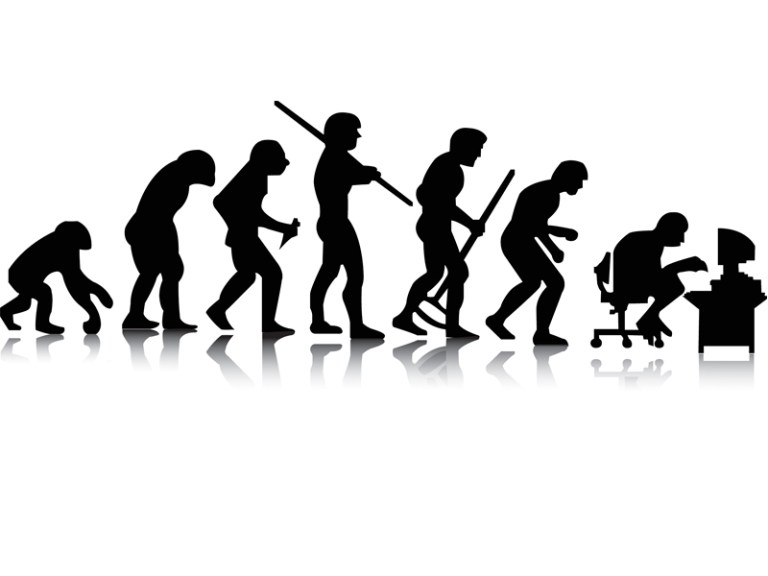
\includegraphics[width=12cm]{images/title.jpg}\cite{titleimg}\\[\bigskipamount]
    \huge
}
\posttitle{
    \end{center}
    \begin{center}
    \Large
    Inwiefern sind genetische Algorithmen ein geeignetes Mittel zur Optimierung der Fahrpläne von Buslinien? \newline \newline Untersuchungen mithilfe einer selbst entwickelten Simulation
    \end{center}
}

% Allgemeine Informationen
\title{5. PK Schriftliche Ausarbeitung}
\author{Amon Benson \& Luca Jungnickel}
\date{}

% Kopf- und Fußzeilen
\pagestyle{scrheadings}
\clearscrheadfoot

\chead{Schriftliche Ausarbeitung - Genetische Algorithmen in der Informatik}
\cfoot{\pagemark}

% Dokumentbeginn
\begin{document}

% Titelseite, Inhaltsverzeichnis, danach bei Seite 1 starten
\maketitle
\newpage

\tableofcontents
\newpage

\setcounter{page}{1}



% GLIEDERUNG
\newpage
\section{Gliederung der Präsentation}

% Aufzählung
\begin{itemize}

\item{Optimierungsproblem}
\begin{itemize}
\item Erklärung unseres Optimierungsproblems (Luca)
\item Erklärung des Aufbaus unserer Simulation (Luca)
\end{itemize}

\item{Genetische Algorithmen}
\begin{itemize}
\item Genetische Algorithmen im Allgemeinen (Amon)
\item Anwendung des Genetischen Algorithmus auf die Simulation (Amon)
\end{itemize}

\item{Ergebnisse}
\begin{itemize}
\item Messreihe zur Effizienz des Genetischen Algorithmus (Luca)
\item Beantwortung der Leitfrage (Amon)
\end{itemize}
\end{itemize}



% DARSTELLUNG DES ARBEITSPROZESS
\newpage
\section{Darstellung des Arbeitsprozesses}



% BEGRÜNDUNG DER THEMENFINDUNG
\subsection{Begründung der Themenfindung}
Da wir uns sehr für Informatik interessieren, sind wir eines Tages auf das Themengebiet der Optimierungsverfahren gestoßen. Hier geht es darum, ein komplexes Problem mittels diverser Algorithmen zu optimieren. Eine mögliche Optimierungsmethode besteht in so genannten genetischen Algorithmen. Hier haben wir uns bei der Themenwahl von einigen interessanten Youtube-Videos inspirieren lassen, welche sich mit dieser Thematik auseinandersetzen. Eines der anschaulichsten Videos behandelt die Optimierung von künstlichen Kreaturen, welche sich mit einfachen Bewegungsfunktionen ausgestattet über eine möglichst weite Strecke bewegen sollten \cite{carykh2015}. Dieses Video zeigt die Funktionsweise von genetischen Algorithmen sehr gut, jedoch gibt es nur einen sehr geringen Bezug zur Realität, da hier nur frei erfundene Kreaturen optimiert wurden. Unser Wunsch war es aber, mithilfe von genetischen Algorithmen etwas Realitätsnäheres zu optimieren.

Das Optimieren von Busrouten im Öffentlichen Nahverkehr in Städten war hier unserer Meinung nach gut geeignet, da sich dieses Problem mit nur wenigen Parametern beschreiben lässt. So ist das Simulieren einer Stadt mit Verkehrsaufkommen zwar komplex, jedoch kann eine Buslinie durch sehr wenige Variablen beschrieben werden, nämlich durch die Startzeit der Busse und der angefahrenen Bushaltestellen. Somit ist der Lösungsraum bei diesem komplexen Problem relativ klein, und so hatten wir den Gedanken, der genetische Algorithmus könne so gut eine sinnvolle Lösung finden.

Damit war unser Thema "`Genetische Algorithmen zur Optimierung vom Öffentlichen Nahverkehr"' gefunden.



% EINORDNUNG IN DEN FACHWISSENSCHAFTLICHEN ZUSAMMENHANG
\subsection{Einordnung in den fachwissenschaftlichen Zusammenhang}

\textit{Lebewesen sind vollendete Problemlöser. In der Vielzahl der Aufgaben, die sie bewältigen, übertreffen die die besten Computerprogamme bei weitem - zur besonderen Frustration der Programmierer, die Monate oder gar Jahre harter geistiger Arbeit für einen Algorithmus aufwenden, währen Organismen ihre Fähigkeiten durch den scheinbar ziellosen Mechanismus der Evolution erwerben.}\\

Das Zitat von J. H. Holland \cite{holland1992} bezieht sich auf evolutionäre Algorithmen. Durch die zunehmende Leistungsfähigkeit von Rechnern sind diese ein neues Optimierungswerkzeug der Numerik geworden. Sie machen sich das Prinzip der biologischen Evolution zum Vorbild. Kleine Veränderungen von Parametern werden zufällig eingeführt. Durch eine Selektion werden die Veränderungen beibehalten, die zu eine Verbesserung bestimmter Aufgaben führen. Über viele Schritte ergibt sich so ein verbessertes Verhalten, ohne dass das zugrundeliegende Prinzip notwendigerweise verstanden sein muss. Ein bekanntes Beispiel \cite{gerdes2004} ist die Optimierung von Flügelformen für Flugzeuge oder ähnliche Probleme in der Aerodynamik.

Erste Ansätze zur evolutionären Optimierung stammen bereits aus den 50er Jahren. \cite{gerdes2004}

Nach unserer Themenwahl haben wir festgestellt, dass tatsächlich auch schon für Probleme der Optimierung von Buslinien genetische Algorithmen verwendet wurden \cite{yu2011}.



% EINGRENZUNG DES THEMAS
\subsection{Konkrete Eingrenzung des Themas und Methodik}
\label{sec:Einschraenkungen_unseres_Themas}
Um festzustellen, inwiefern genetische Algorithmen Fahrpläne von Buslinien optimieren können, hatten wir die Idee, eine eigene Simulation zu schreiben, welche wir dann mit unserem erstellten genetischen Algorithmus koppeln. Dadurch können wir so präzise wie möglich verstehen, wie ein genetischer Algorithmus funktioniert und sehr genaue Einstellungen und Veränderungen der Simulation vornehmen. Somit ist der Lerneffekt am höchsten. 

In unserer Simulation haben wir das Programm \textit{Eclipse} verwendet, mit dem Java-Programmierung durchgeführt werden kann. Diese Programm ist weit verbreitet und kostenlos erhältlich. Wir haben es auf normalen Windows-Notebooks eingerichtet. Die Simulation wurde auf der CPU durchgeführt.
Die aktuelle Version unserer Applikation kann auf GitHub als Eclipse-Projekt heruntergeladen werden \cite{trafficsimGitHub}.

Nachdem wir uns ausführlich über die Funktionsweise von genetischen Algorithmen informiert hatten, mussten wir konkrete Einschränkungen und Überlegungen machen, wie komplex unsere Simulation und das gesamte Projekt werden soll. Somit haben wir als Erstes entschieden, wie die Simulation aufgebaut ist und wie der genetische Algorithmus die Simulation verwendet. So haben wir festgelegt, dass die Simulation einer Stadtfläche mithilfe einer gerasterten Karte dargestellt werden kann, wobei jede Kachel quadratisch ist. Eine Kachel kann entweder eine Gebäude oder eine Straße sein (s. Abb.~\ref{fig:tileexample}).

\begin{figure}[H]
    \centering
    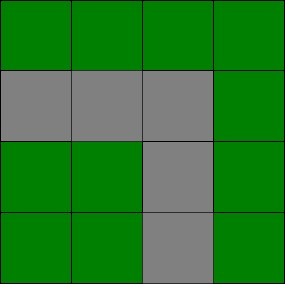
\includegraphics[width=0.4\linewidth]{images/tilestreet.jpg}
    \caption{Darstellung der Stadtfläche durch Rasterkarte. Eine grüne Kachel repräsentiert ein Haus mit Verkehrsaufkommen, eine dunkelgraue Kachel ist eine Straße}
    \label{fig:tileexample}
\end{figure}

Uns war von Anfang an bewusst, dass dies eine Einschränkung ist, da gewöhnliche Straßennetze nicht notwendigerweise rechteckig aufgebaut sind. Oft ist dies jedoch der Fall und wir mussten diese Einschränkung vornehmen, da es deutlich zu kompliziert gewesen wäre, ein realistisches Verkehrsnetz in die Simulation zu implementieren.

Eine weitere Einschränkung ist die vereinfachte Darstellung des Verkehrs. Wir haben uns dafür entschieden, dass Verkehrssystem so einfach wie möglich zu halten. Konkret ist damit gemeint, dass wir komplett auf Spuren, Ampeln, Einbahnstraßen o.ä. verzichtet haben. Außerdem behindern sich entgegenkommende Fahrzeuge nicht.
Der einzige Parameter, welcher den Verkehr beeinflusst, ist die Geschwindigkeit der jeweiligen Straßenkachel. Ein Bus nimmt sofort den Geschwindigkeitswert der befahrenden Straße an. Damit lässt sich die Realität auch sehr gut nachbilden, da für eine Straße die in der Realität durchschnittlich gefahrene Geschwindigkeit als dauerhafter Geschwindigkeitswert der Simulation gelten kann. So können Straßen mit hohem Verkehrsaufkommen nachgebildet werden, indem die Geschwindigkeit der Straße in der Simulation geringer gesetzt wird. Auch sehr kleine Straßen, in denen baulich bedingt sehr langsam gefahren werden muss, können durch einen geringen Geschwindigkeitswert nachgestellt werden. Straßen, auf denen nur wenig Verkehr herrscht, jedoch sehr schnell gefahren werden darf, können durch einen hohen Geschwindigkeitswert in der Simulation eingefügt werden.

Diese Form der Vereinfachung hat jedoch auch eine Grenze. Wenn eine hohe Anzahl an Bussen regelmäßig über eine Straßenkachel fahren (zum Beispiel 10 Busse pro 1 simulierten Minute), dann würde sich in der Realität das Verkehrsaufkommen auf dieser Straße sehr erhöhen und somit würde die Durchschnittsgeschwindigkeit geringer werden. Da in der Simulation die Geschwindigkeit einer Straße aber immer konstant ist, wird nicht betrachtet, inwiefern die fahrenden Busse einen Einfluss auf die Verkehrsdichte haben.
Jedoch ist dieses nichtlineare Problem unserer Meinung nach vernachlässigbar, da in der Realität die Verkehrsdichte durch Busse nicht wesentlich erhöht wird. Selten führen Busse zum "`Verstopfen"' einer Straße, der Individualverkehr ist hier viel schwerwiegender.

Um die Komplexität unserer Simulation nicht noch weiter zu steigern, mussten wir uns zu Beginn das Problem der Wegfindung von Personen genau überlegen. In der Simulation werden nämlich zufällig Personen erzeugt, welche von einem zufälligen Start zu einem zufälligen Ziel gefahren werden wollen. Dafür muss jede Person ermitteln, mit welchen Buslinien sie fahren und an welchen Bushaltestellen sie umsteigen muss. Da unser Fokus auf die Optimierung der Buslinien mithilfe genetischen Algorithmen lag, haben wir uns entschieden, den Wegfindungsalgorithmus zu vereinfachen.
Konkret heißt dies, das der Wegfindungsalgorithmus als Route immer den von der Strecke her kürzesten Weg ermitteln wird, unabhängig davon, wie oft umgestiegen werden muss und wie sinnvoll dieser Weg eigentlich ist.

\begin{figure}[H]
    \centering
    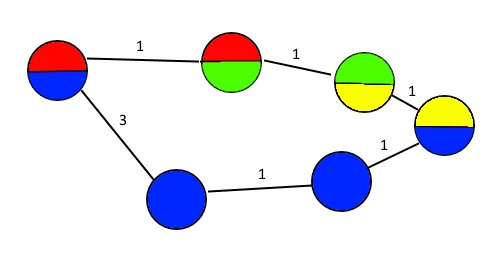
\includegraphics[width=0.7\linewidth]{images/pathfind.jpg}
    \caption{Skizze der vereinfachten Wegfindung. Die Kreise repräsentieren Stationen, die Farben verschiedene Buslinien. Ziel ist es, möglichst schnell vom Startpunkt (ganz linker Kreis) zum Zielpunkt (ganz rechter Kreis) zu gelangen. Die jeweilige Zahl zwischen den Kreisen gibt die zurückzulegende Strecke des Busses an, um zur nächsten Station zu fahren.}  \label{fig:pathfindexample}
\end{figure}

Die Abbildung \ref{fig:pathfindexample} veranschaulicht das Problem. Der implementierte Wegfindungsalgorithmus wird als Strecke zwischen dem linken und dem rechten Punkt die obere Route wählen, da die Strecke hier insgesamt 3 beträgt. Der untere Weg hat eine Strecke von 5, jedoch kann die Person das Ziel mit nur einem Bus erreichen. In der oberen Route muss die Person von der roten zur grünen zur gelben Buslinie umsteigen, in der Realität ist diese Strecke natürlich deutlich schlechter und man würde die blaue Buslinie favorisieren. Da diese genaue Art der Wegfindung jedoch so nicht implementiert wurde, werden in der Simulation teilweise komplizierte Routen gefunden. In einer Erweiterung des Algorithmus könnte eine Favorisierung von Strecken mit wenigen Umstiegen zum Beispiel durch einen Gewichtungsfaktor eingebaut werden.\\

Der von uns programmierte Algorithmus basiert auf der Quelle \cite{gerdes2004}. Teilweise konnten Java-Routinen aus \cite{gerdes2004}, \cite{jacobson2015} und \cite{selzam2006}. In diesen Quellen finden sich auch Dokumentationen, auf die hier nicht im Detail eingegangen werden kann.

In Bezug auf den genetischen Algorithmus entschieden wir uns dazu, die Chromosomen einzelner Individuen in Abschnitte zu unterteilen. Das erlaubte uns nun, die Wertebereiche einzelner Abschnitte unabhängig voneinander festzulegen; Der Abschnitt, der die Stationen kodiert, kann so booleanische Werte für die Zustände "`Station"' und "`keine Station"' enthalten, während die Abschnitte, die die Busabfahrtszeiten festlegen, als Ganzzahlen interpretiert werden. Auch haben wir auf die Implementierung unterschiedlicher Mutations- und Crossover-Methoden \cite{gerdes2004} verzichtet und verwenden in jeder Generation der Einfachheit halber ein und dieselbe Methode.

Der Hauptteil der Arbeit für die Präsentation war die Programmierung und der Test des Algorithmus. In der Präsentation wird dieser motiviert und erklärt. Zusätzlich wird die Simulation live präsentiert und anschließend diskutiert.



% ARBEITSPLAN
\newpage
\section{Arbeitsplan}

Im Folgenden wird der Arbeitsplan in kompakter Form als Tabelle dargestellt.

% Arbeitsablauf-Tabelle
\newlength\tabledate
\newlength\tablecontent
\newlength\tablerow
\setlength{\tabledate}{3.5cm}
\setlength{\tablecontent}{10.5cm}
\setlength{\tablerow}{5.1cm}
\begin{longtable}{p{\tabledate}|p{\tablerow}|p{\tablerow}} % Datumspalte fixieren, andere Spalten ausdehnen

\textbf{Datum} & \textbf{Amon} & \textbf{Luca} \\
\hline

April 2017 & \multicolumn{2}{p{\tablecontent}}{Hier kam zum ersten Mal die Idee auf, genetische Algorithmen als Hauptbestandteil unserer Präsentationsprüfung zu verwenden. Wenig später einigten wir und dann auch schon auf das jetzige Thema: Die Planung von Busrouten mithilfe eines genetischen Algorithmus. Auch ein erstes Treffen mit dem Fachlehrer in Bezug auf die Realisierbarkeit dieses Themas fand im April statt.}\\
\hline

21. April 2017 & \multicolumn{2}{p{\tablecontent}}{Erstes Treffen, um die Aufteilung der Programmieraufgaben zu besprechen. Außerdem richteten wir eine Git-Repository ein, mithilfe derer wir unser Projekt gemeinsam bearbeiten und synchronisieren konnten.}\\
\hline

Mai bis August 2017 & Graphische Einarbeitung der Simulation. Anzeige der Tile-basierten Stadt, der Events, Personen und aktiven Buslinien. & Programmieren der Simulation. Gegen Ende August funktionierten die Wegfindungsalgorithmen noch nicht, wir verwendeten also fixe Buslinien. Das Transportieren von Personen war allerdings schon möglich.\\
\hline

2. September 2017 & \multicolumn{2}{p{\tablecontent}}{Zusammenführen der Ergebnisse.}\\
\hline

20. September 2017 & \multicolumn{2}{p{\tablecontent}}{Treffen mit dem betreuenden Fachlehrer, um den Fortschritt unseres Projektes zu besprechen.}\\
\hline

27. September 2017 & \multicolumn{2}{p{\tablecontent}}{Treffen mit dem betreuenden Fachlehrer. Besprechen der vorläufigen Gliederung und des Inhalts unseres Vortrags.}\\
\hline

4. November 2017 & \multicolumn{2}{p{\tablecontent}}{Besuch der Code-Night am Hasso Plattner Institut. Ziel war es, eine Nacht lang gemeinsam mit anderen Informatik interessierten Schülern an einem Projekt zu arbeiten. Dies half uns auch in Bezug auf unsere Präsentationsprüfung, da man einiges über die Arbeitsteilung im Team und die Nutzung von GitHub \cite{trafficsimGitHub} für eine gemeinsame Projektverwaltung lernte. In der Code Night hat unser Team den \textit{ersten Platz} erzielt.}\\
\hline

14. November 2017 & \multicolumn{2}{p{\tablecontent}}{Letztes Treffen mit dem betreuenden Fachlehrer vor Abgabe des Exposés.}\\
\hline

7. Januar 2018 & Entwicklung eines genetischen Algorithmus in Java, unabhängig von unserer Simulation. & Implementierung der Wegfindungsalgorithmen in die Simulation.\\
\hline

20. Januar 2018 & Einarbeiten des genetischen Algorithmus in die Simulation. & Fertigstellung der Simulation, Erstellung des "Blueprint-Converters". Dieser wandelt einen Chromosomensatz (bestehend aus Ganzzahlen) in einen Plan zum Erstellen der Buslinien um. Dieser Plan kann dann in der Stadt simuliert werden.\\
\hline

28. Januar 2018 & Anzeigen des genetischen Stammbaums. Alle Individuen mit Verbindungen zu ihren Eltern werden in einem separaten Fenster angezeigt, aktueller Fortschritt des genetischen Algorithmus kann simuliert werden. & Beheben der letzten Fehler in den Wegfindungsalgorithmen der Simulation.\\
\hline

6. Februar 2018 & \multicolumn{2}{p{\tablecontent}}{Implementierung einer Fitness-Funktion. Diese wertet eine Simulation aus und gibt dem Individuum seinen Fitness Wert. Außerdem führten wir erste erfolgreiche Tests des gesamten Programms durch.} \\
\hline

11. Februar 2018 & \multicolumn{2}{p{\tablecontent}}{Auswertung weiterer Versuchsreihen, erste Tests an einer nachgebildeten Karten von Manhattan.} \\
\hline

15. Februar 2018 & \multicolumn{2}{p{\tablecontent}}{Letztes Treffen mit dem betreuenden Fachlehrer vor Abgabe der schriftlichen Ausarbeitung.} \\
\hline

\end{longtable}



% REFLEXION AMON
\newpage
\section{Individuelle Reflexion}
\subsection{Amon}
Die Arbeit an unsere Präsentationsprüfung lieferte mir einen umfangreichen Einblick in die Welt der evolutionären Algorithmen.\\

Schon vor der Themenwahl hatte ich bereits von genetischen Algorithmen gehört, besonders hilfreich waren dort einige Videos auf YouTube \cite{carykh2015}, die einen sehr leicht verständlichen, aber nur groben Überblick über dieses Gebiet geben.

So fiel die Entscheidung für ein Themenfeld der Präsentationsprüfung auf genetische Algorithmen. Die erste schwierige Frage war dann die Einigung auf ein konkretes Thema. Meine Idee war es, genetische Algorithmen mit Musik zu verknüpfen, d. h. zum Beispiel eine Software zu entwickeln, die automatisch Akkorde oder Melodien generiert. Auch wenn das sicherlich eine nette Spielerei gewesen wäre, fehlt hier doch etwas der Bezug zur realen Welt bzw. ein sinnvoller Anwendungszweck. Luca brachte dann den Vorschlag, die Infrastruktur einer Stadt genetisch generieren zu lassen.

Relativ schnell wurde uns bewusst, dass wir dieses Thema extrem eingrenzen müssten. Somit begrenzten wir die Simulation auf Buslinien. Danach überlegten wir uns, wie eine Simulation aufgebaut sein müsste und entwarfen Pläne für das Busroutensystem und die Wegfindung der Personen. Die Aufteilung und Zusammenarbeit gelang vollkommen problemlos. Luca beschäftigte sich zunächst hauptsächlich mit der Programmierung der Simulation, während ich mich um deren graphische Implementierung und später um die Programmierung der genetischen Algorithmen kümmerte. Dieses Prinzip der Trennung von "`Core-Anwendung"' und Grafik stammt aus unserer Quelle über objektorientierte Programmierung von Balzert \cite{balzert2014}, welche mir auch unabhängig von unserer Präsentationsprüfung sehr bei der strukturierten und organisierten Programmierung half.

Ich besorgte mir Literatur zur Programmierung von genetischen Algorithmen \cite{selzam2006,jacobson2015} und programmierte einige Beispiele aus \cite{jacobson2015} nach, bis ich dann Anfang Januar 2018 begann, den genetischen Algorithmus für unser Projekt zu erstellen.\\

Es beruhigt mich auf jeden Fall, dass unser Projekt letzten Endes an kleineren Städten sehr erfolgreiche Ergebnisse liefert. Es ist jedoch etwas Schade, dass wir am Schluss nur wenig Zeit zum "`Experimentieren"' hatten. Auch musste stellenweise mehr Wert auf Schnelligkeit zur Erreichung eines konkreten Ergebnisses als auf höchste Sorgfalt (Kommetierung, Eleganz der Umsetzung) gelegt werden.



% REFLEXION LUCA
\newpage
\subsection{Luca}
Die Arbeitsteilung zwischen Amon und mir hat hervorragend funktioniert. Hier hatten wir bereits Erfahrung, da wir gemeinsam die MSA Präsentation gemacht haben und schon dort die Zusammenarbeit sehr gut funktioniert hat.

Zu Beginn haben Amon und ich das Thema sinnvoll eingeschränkt. So hatten wir zuerst die Idee, eine ganze Infrastruktur in einer Stadt zu optimieren, also zum Beispiel auch zu optimieren, wo Straßen gebaut werden, Siedlungen geschaffen werden oder ähnliches. Schnell haben wir jedoch gemerkt, dass dies zu komplex wird und wir uns auf eine einfachere Optimierung beschränken sollten. So haben wir uns schließlich geeinigt, '`nur'' die Buslinien in einer Stadt mithilfe einer selbstentwickelten Simulation zu optimieren.\\

In der Simulation habe ich zunächst die "`Core"'-Anwendung programmiert, also die rechnerische Grundlage ohne eine grafische Darstellung. Amon hat sich zuerst auf die Programmierung der Grafik und später auf die Programmierung des genetischen Algorithmus fokussiert. Dabei mussten viele Entscheidungen, welche die Funktion der Simulation betreffen, gefällt werden. So habe ich mich unter anderem entschieden, die Wegfindungsalgorithmen in der Simulation zu vereinfachen, da der Fokus unserer Arbeit die Optimierung mithilfe genetischer Algorithmen ist, und nicht die der Wegfindungsalgorithmen (siehe Abschnitt \ref{sec:Einschraenkungen_unseres_Themas}). Abschließend betrachtet war das eine sehr gute Entscheidung, da der Auswirkungen der Vereinfachung verkraftbar sind und wir uns so auf die gründliche Implementierung des genetischen Algorithmus konzentrieren konnten.

Die Quellenwahl sowie Recherche ist mir sehr leicht gefallen, so hatte ich bereits Erfahrung in der Einbindung von sog. Third-party-libraries, also der Verwendung von fremden Bibliotheken in der Programmierung. Dadurch konnte ich mich auf die eigentliche Programmierung konzentrieren. Außerdem gibt es zu der Thematik der genetischen Algorithmen sehr gute und ausführliche Literatur, welche zwar eigentlich auf Universitätsniveau ist, jedoch in den meisten Punkten auch verständlich ist. Ein Problem für mich war, die beschriebene Mathematik in meiner Hauptquelle \cite{gerdes2004} zu verstehen. Diese ist auf Universitätsniveau und so sehr verschieden zu der Art von Mathematik, welche man in der Schule kennenlernt. Nichtsdestotrotz konnte mir diese Quelle einen sehr tiefen Einblick in dieses Thema geben und war so für mich Grundlage in der Entwicklung des genetischen Algorithmus.\\

Abschließend lässt sich die Planung und Umsetzung des Projektes als sehr erfolgreich betrachten. So haben wir es geschafft, dieses komplexe Projekt umzusetzen und ein funktionierendes Ergebnis vorzeigen zu können. Zusätzlich haben wir ein unserer Meinung interessantes Thema ausgesucht, an dem wir Spaß hatten, zu arbeiten. Dadurch haben wir uns intensiv mit dem Themengebiet auseinandergesetzt und sehr viel gelernt. Auch für die Zukunft hat mir dieses Thema einiges gebracht, da ich voraussichtlich technische Informatik studieren möchte und es so sehr sinnvoll ist, bereits einen Einblick in ein Themengebiet der Informatik zu erhalten. Ich habe ausführlich gelernt, wie genetische Algorithmen funktionieren und wie man diese mit einfachen Methoden effektiv gestalten kann, wie große Softwareprojekte zu strukturieren sind und wie man gemeinsam an einer Software arbeitet und dies koordiniert. Auch wenn letzteres nicht explizit etwas mit unserer Fragestellung zu tun hat, ist auch dieses Wissen in der Informatik sehr wichtig.



% LITERATURVERZEICHNIS
\newpage
\section{Literaturverzeichnis}

% Show the bib
\renewcommand{\section}[2]{} % No title for the bib
\nocite{*}
\printbibliography



% Das war's. Yay!
\end{document}